\subsection{Mønstergenkendelse}

\begin{center}
	\textit{''A pattern is an arrangement of discriptors''}
\end{center}

En \textit{feature} er et ofte brugt navn for en \textit{descriptor}.\\

\subsubsection{Pattern Class}

En \textit{pattern class} er beskrevet som en familie af mønstre som alle deler nogle fælles attributter/properties.

Pattern classes er skrevet som: 

\begin{equation}
w_1, w_2,...w_W
\end{equation}

Hvor $W$ er antallet af klasser.

\subsubsection{Pattern Vector}

Bruges til at opstille \textit{descriptors}/attributterne. Her er $n$ antallet af attributter og hver $x_i$ er en attribut.

\begin{equation}
\mathbf{x} = \begin{bmatrix}x_1\\ x_2\\ \vdots \\ x_n\end{bmatrix}
\end{equation}

For tilfældet med blomsterne (Figur~\ref{fig:iris-graph}) har vi to attributter, som vi kan udtrykker ved følgende vektor vist i Ligning~\ref{eq:pattern-vector-iris}. Her er $x_1$ og $x_2$ længde og bredde af kronbladene også plottet i Figur~\ref{fig:iris-graph}.

\begin{equation}\label{eq:pattern-vector-iris}
\mathbf{x} = \begin{bmatrix}x_1\\ x_2\end{bmatrix}
\end{equation}

\begin{figure}[H]
	\centering
	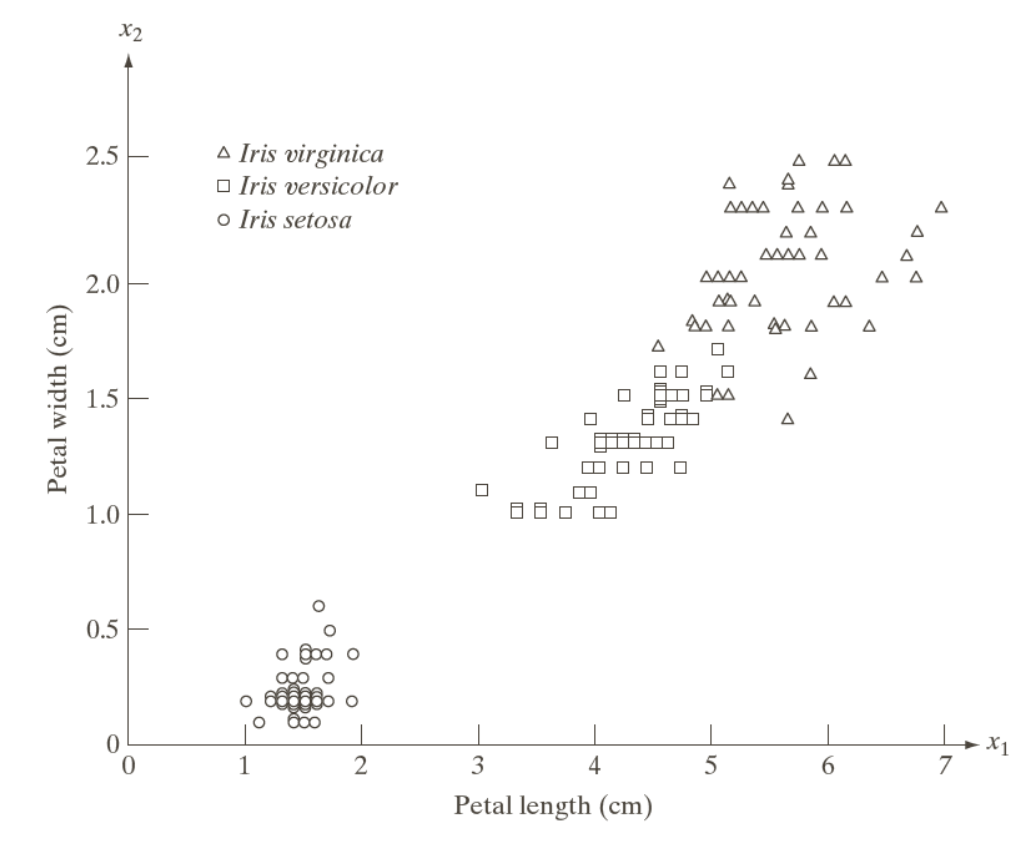
\includegraphics[width=0.9\linewidth]{figs/spm12/iris-graph}
	\caption{Tre typer af Iris blomster beskrevet ved to målinger.}
	\label{fig:iris-graph}
\end{figure}

\subsubsection{Teknikker}

Bogen nævner to primær metoder for mønstergenkendelse, som bruger forskellig information til at lave pattern klasserne.  

\begin{itemize}
	\item Kvantitativ information.
	\item Strukturelle forhold.
	\item Tree descriptions.
\end{itemize}

\paragraph{Kvantitativ}

Bruger en vektor som tidligere nævnt til at plotte typer i et diagram som det på Figur~\ref{fig:iris-graph}.

\paragraph{Strukturelle}

Vil eksempelvis primært bruges til at genkende fingeraftryk, hvor de er linjerne indbyrdes forhold som kan bruges til at finde ligheder.

\paragraph{Tree}

En hierarkisk inddeling af billedet i komponenter. Figur~\ref{fig:tree-town-image} viser træet for en by (bybillede i bogen, ikke medtaget). 

\begin{figure}[H]
	\centering
	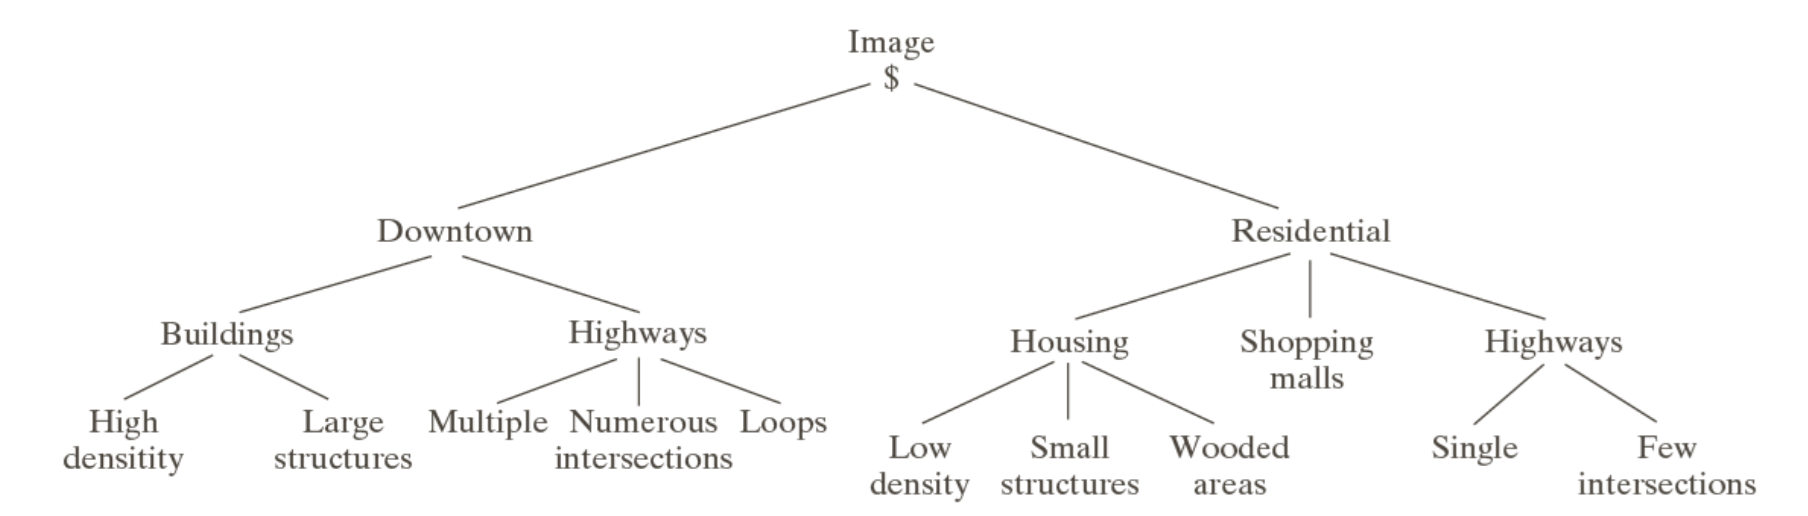
\includegraphics[width=\linewidth]{figs/spm12/tree-town-image}
	\caption{Tree descriptors brugt til at opløse et billede af en by.}
	\label{fig:tree-town-image}
\end{figure}


